\section{Parking Lot Generation}

Once the plot generation is finished the parking lot generation starts working towards filling some of the generated plots with parking lots.

The generated parking lots consist of either two or four columns of parking spaces (see Figure ~\ref{fig:sizebased}).
\begin{figure}[H]
   \centering
   \begin{subfigure}[b]{0.485\textwidth}
     \frame{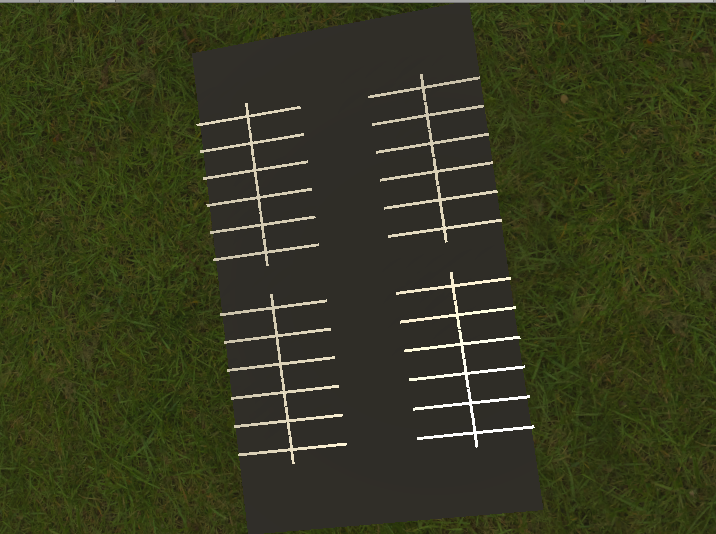
\includegraphics[width=\textwidth]{figure/fourcol}}
     \caption{Large parking lot consisting of four columns.}
   \end{subfigure}
   \quad
   \begin{subfigure}[b]{0.45\textwidth}
     \frame{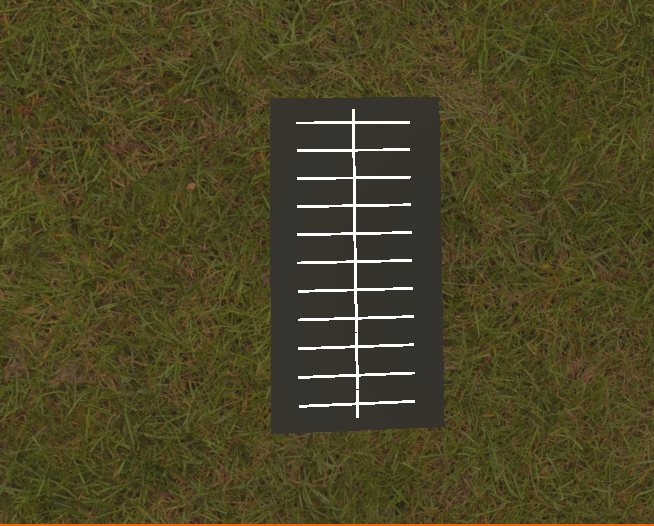
\includegraphics[width=\textwidth]{figure/twocol}}
     \caption{Small parking lot consisting of two columns.}
   \end{subfigure}
     \caption{Two examples of different sized parking lots created by the generator.}
   \label{fig:sizebased}
 \end{figure}
These parking lots are generated by calculating the largest possible rectangle inside a polygon, and then generating a parking lot inside them.
The number of columns is based on the size of the approximated rectangle, such that a larger rectangle will always result in parking lot with four columns, and a smaller rectangle will always result in a parking lot with two.
Inside the larger rectangles the columns will be inset from the corners of the rectangle and then parking lots will be generated in a shape like this ~Figure\ref{fig:bigparking}.
\begin{figure}[H]
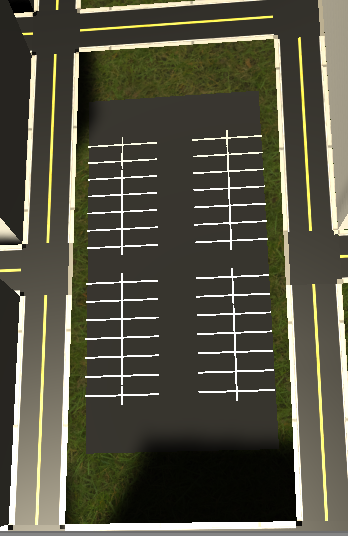
\includegraphics[width=\linewidth]{figure/bigp.PNG}
\caption{Example of four column parking lot.}
\label{fig:bigparking}
\end{figure}
For the smaller rectangles however the parking lots will be generated starting from the center of the rectangle like this ~Figure\ref{fig:smallparking}.
\begin{figure}[H]
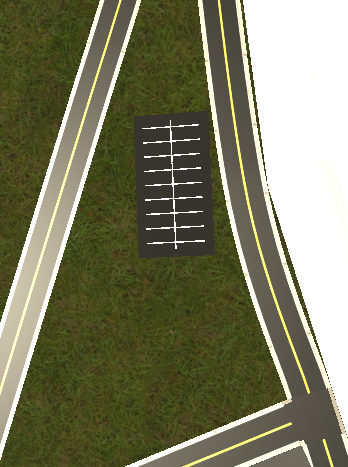
\includegraphics[width=\linewidth]{figure/smallp.PNG}
\caption{Example of two column parking lot.}
\label{fig:smallparking}
\end{figure}

Having the parking lots be of at least two different shapes gives some more variety, but the decision to do this was also based on real-world parking lots (see Figure~\ref{fig:parkings}).
From the left image it is obvious that not having a road separate the columns would make it possible for a car to be entirely parked in and unavailable to move. The right image however has a more interesting shape.
The parking lot in the center of it is shaped in the two-column style, however the surrounding rectangle is large enough that cars can easily drive around and not be blocked by parked cars. 
\begin{figure}[H]
   \centering
   \begin{subfigure}[b]{0.55\textwidth}
     \frame{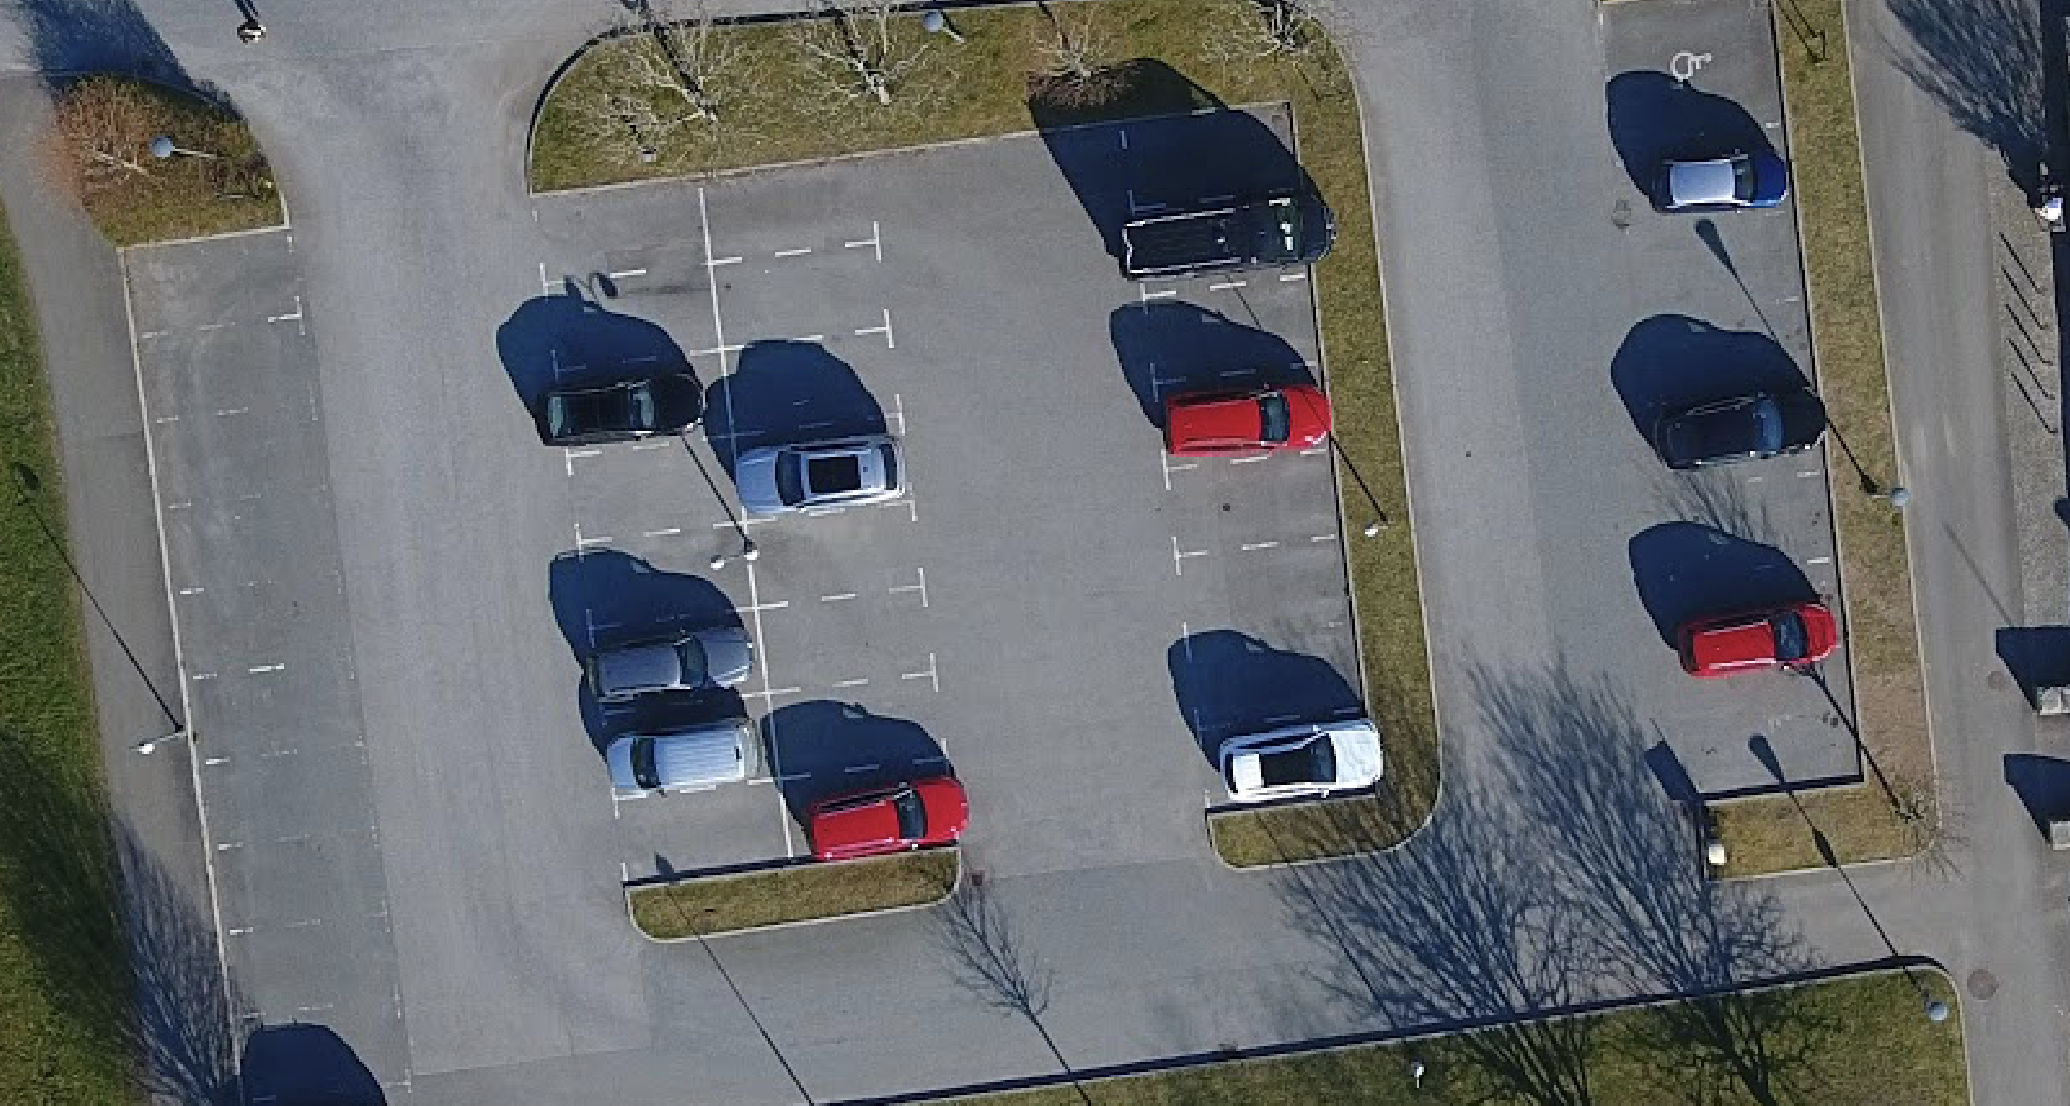
\includegraphics[width=\textwidth]{figure/parking1}}
   \end{subfigure}
   \quad
   \begin{subfigure}[b]{0.395\textwidth}
     \frame{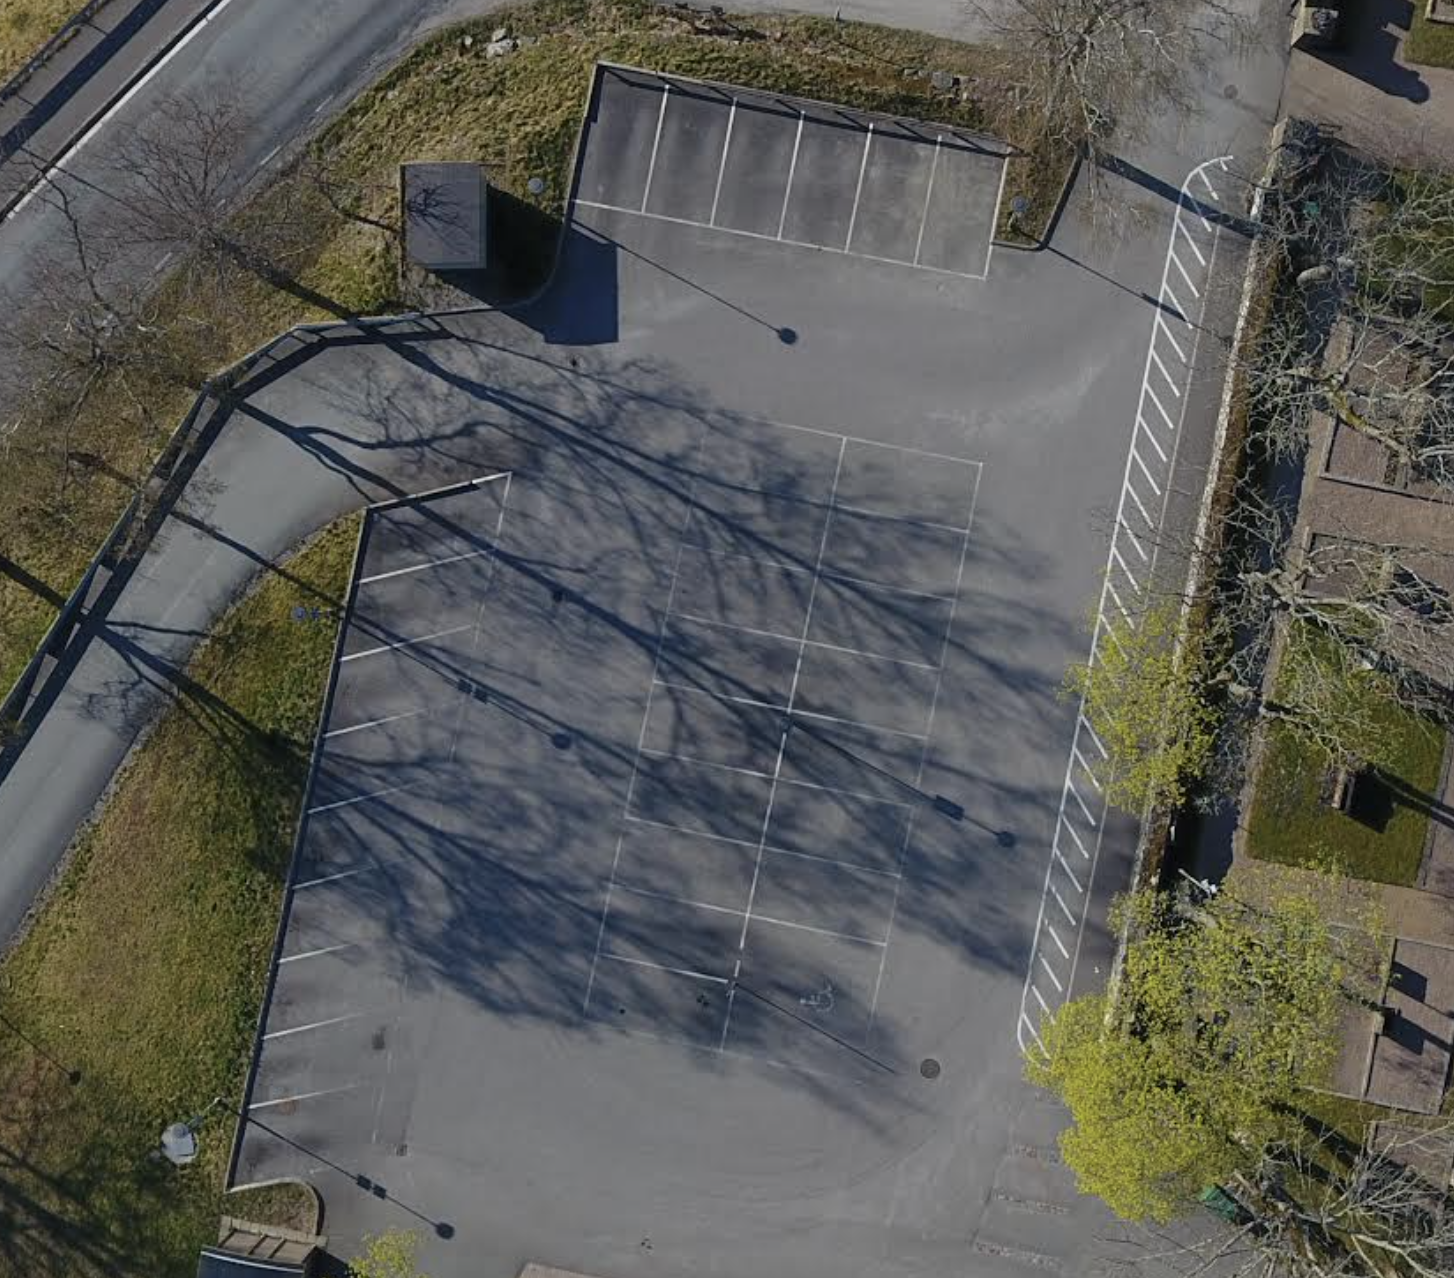
\includegraphics[width=\textwidth]{figure/parking2}}
   \end{subfigure}
   \caption{Two examples of parking lots observed by the project group, showcasing the rectangular shapes mentioned above.}
   \label{fig:parkings}
 \end{figure}









